% !TEX TS-program = xelatex
% !TEX encoding = UTF-8 Unicode 

% \documentclass[AutoFakeBold]{LZUThesis}
\documentclass[AutoFakeBold]{LZUThesis}
\usepackage{multirow}
\usepackage{threeparttable}
\CTEXsetup[name={第,部分}]{chapter}
\lstset{
language = MATLAB,
backgroundcolor=\color{white},   % choose the background color; you must add \usepackage{color} or \usepackage{xcolor}  
basicstyle=\footnotesize,        % the size of the fonts that are used for the code  
breakatwhitespace=false,         % sets if automatic breaks should only happen at whitespace  
breaklines=true,                 % sets automatic line breaking  
captionpos=bl,                    % sets the caption-position to bottom  
% commentstyle=\color{green},    % comment style  
% deletekeywords={...},            % if you want to delete keywords from the given language  
% escapeinside={\%*}{*)},          % if you want to add LaTeX within your code  
extendedchars=true,              % lets you use non-ASCII characters; for 8-bits encodings only, does not work with UTF-8  
frame=shadowbox,                    % adds a frame around the code  
keepspaces=true,                 % keeps spaces in text, useful for keeping indentation of code (possibly needs columns=flexible)  
keywordstyle=\color{blue},       % keyword style  
% language=Python,                 % the language of the code  
morekeywords={*,...},            % if you want to add more keywords to the set  
numbers=left,                    % where to put the line-numbers; possible values are (none, left, right)  
numbersep=5pt,                   % how far the line-numbers are from the code  
numberstyle=\tiny\color{gray}, % the style that is used for the line-numbers  
rulecolor=\color{black},         % if not set, the frame-color may be changed on line-breaks within not-black text (e.g. comments (green here))  
showspaces=false,                % show spaces everywhere adding particular underscores; it overrides 'showstringspaces'  
showstringspaces=false,          % underline spaces within strings only  
showtabs=false,                  % show tabs within strings adding particular underscores  
stepnumber=1,                    % the step between two line-numbers. If it's 1, each line will be numbered  
stringstyle=\color{orange},     % string literal style  
tabsize=2,                       % sets default tabsize to 2 spaces  
% title=signalAnalysis.m           % show the filename of files included with \lstinputlisting; also try caption instead of title  
}  

\begin{document}
%=====%
%
%封皮页填写内容
%
%=====%

% 标题样式 使用 \title{{}}; 使用时必须保证至少两个外侧括号
%  如: 短标题 \title{{第一行}},  
% 	      长标题 \title{{第一行}{第二行}}
%             超长标题\tiitle{{第一行}{...}{第N行}}

\title{{747喷气式飞机偏航阻尼器设计的自我理解}}



% 标题样式 使用 \entitle{{}}; 使用时必须保证至少两个外侧括号
%  如: 短标题 \entitle{{First row}},  
% 	      长标题 \entitle{{First row}{ Second row}}
%             超长标题\entitle{{First row}{...}{ Next N row}}
% 注意:  英文标题多行时 需要在开头加个空格 防止摘要标题处英语单词粘连.

\author{\CJKfontspec{楷体}李文涛}
\major{电子信息基地班}
\college{320200928101}
\grade{2020级}



\maketitle
\frontmatter

%中文摘要
\ZhAbstract{
该篇747喷气飞机偏航阻尼器的设计思路很好地向我展现了自动控制系统的一般设计过程,令我更好地理解了自动控制理论在生活中的应用,同时也让我将书本上的知识有了实际的依托,对刚刚学的根轨迹有了更深的认识。在这篇论文里,我将以我的理解来叙述整个偏航阻尼器的设计过程。
}{阻尼器、根轨迹、设计}




%生成目录
% \tableofcontents
% \addcontentsline{toc}{chapter}{目录}
% \thispagestyle{empty}


%文章主体
\mainmatter

\chapter{设计过程}

\section{明确目标}
首先第一步就是将现实的物理问题抽象成数学问题。
在这里,之前的研究人员已经给出了简化的飞机巡航稳定方程,如下所示,

\begin{equation}
\frac{dx}{dt} =Ax+Bu
\end{equation}
\begin{equation}
y=Cx+Du
\end{equation}
该方程有两个输入分别为飞机方向舵和副翼的偏转,同时有四个状态值分别为Beta(侧滑角),phi(倾斜角),偏航率,滚转率,这量化表示了飞机的飞行姿态和是否稳定飞行的状态。
接着我们将ABCD四个值输送给matlab,利用SS命令建立我们的飞机飞行的数学模型。

对于这个控制系统模型,在实际情况下有着对应,绘制出这个模型的零点和极点,在这里两个极点对应的是飞机的荷兰滚运动姿态,飞机的这个滚动特性是判定飞机操纵品质的一个重要指标,一般会通过荷兰滚实验来得到飞机的动态特性的阻尼比ζ、无阻尼自振频率ωn和阻尼ξ等,以检查飞机动态特性是否满足相应标准和规范的要求。

在此次设计中,我们的零极点图显示在荷兰滚情况下阻尼不够,我们的任务就是设计一个阻尼器来补偿这两个极点的阻尼。
典型的偏航阻尼器是用偏航速率作为感知输出和方向舵作为输入来设计的。我们就针对这个来设计我们的阻尼器。

\section{调整阻尼器参数}
在例子中我们是通过尝试先确定反馈的正负,通过观察根轨迹图,发现当使用积极反馈时,根轨迹处于左半平面,符合系统稳定的要求(图1.1)。

\begin{figure}[htbp]
    \centering
    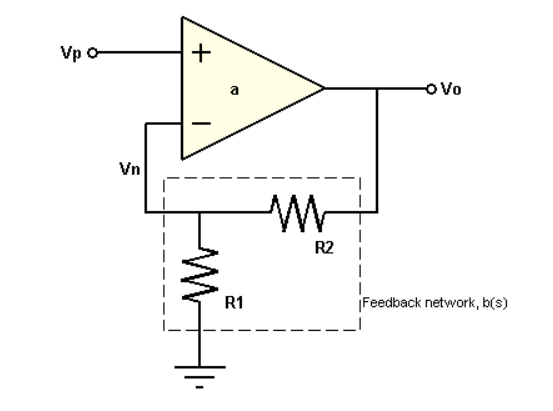
\includegraphics[keepaspectratio,width=500pt]{1.png}
    \caption{有阻尼器的情况下系统的根轨迹}
\end{figure}

通过移动根轨迹上的点来跟踪增益和阻尼值,这里我们取增益K=2.85时,可实现的最佳闭环阻尼约为0.44。
这时关闭掉反馈回路来看看加上我们设计的阻尼器模型后,偏航率对于来自方向舵的冲击的响应(图1.2)

\begin{figure}[htbp]
    \centering
    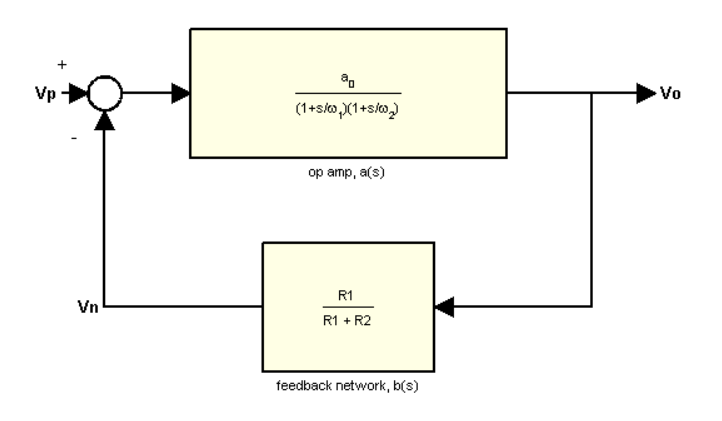
\includegraphics[keepaspectratio,width=500pt]{2.png}
    \caption{偏航率对于来自方向舵的冲击的响应}
\end{figure}

效果还是不错的。
接下来检测副翼的响应状况,闭合环路,反馈回路包括设备的输入1和输出1(图1.3):

\begin{figure}[htbp]
    \centering
    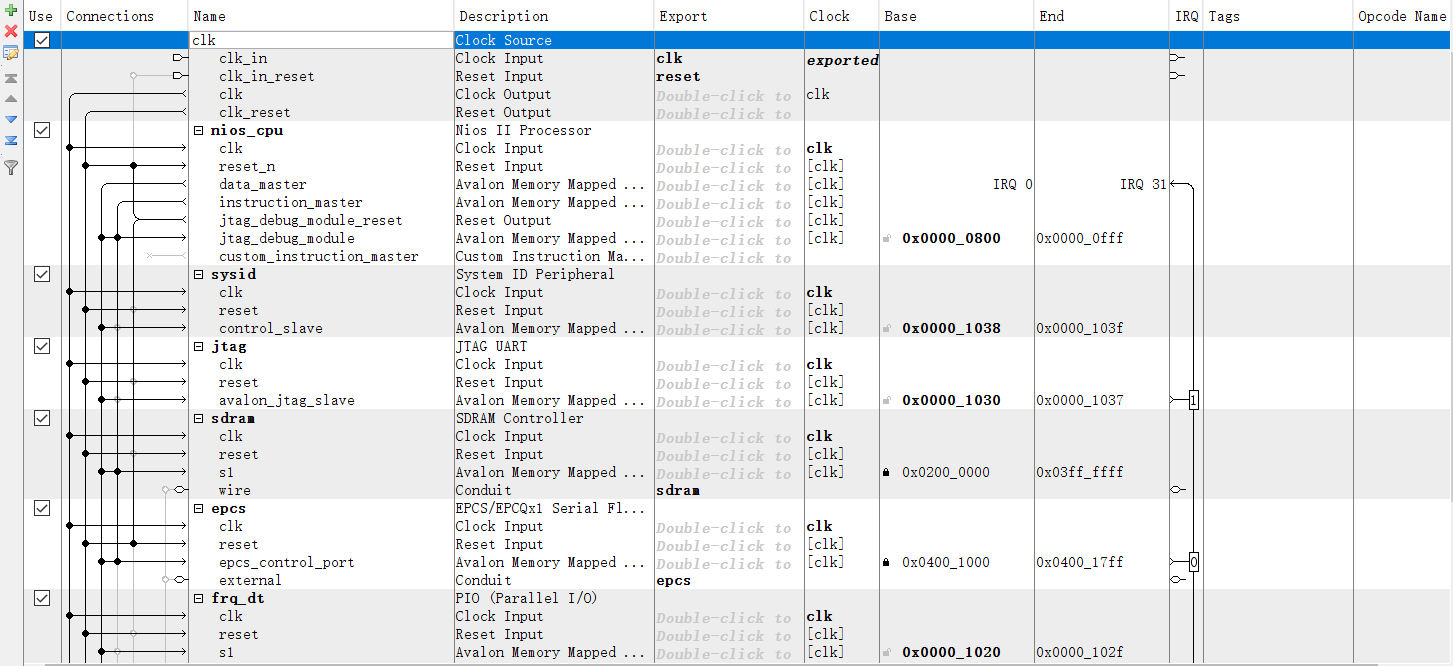
\includegraphics[keepaspectratio,width=500pt]{3.png}
    \caption{闭合回路下副翼的冲击响应}
\end{figure}

可以看到对于偏航率来说,加入我们设计的阻尼器后得到了有效的快速效应及抑制。

\section{按需改进}
但是问题随之出现,我们观察到移动副翼时,系统不再像正常飞机那样继续倾斜,即过度稳定了the spiral mode(螺旋模式),即在没有恒定的副翼输入的情况下倾斜和转向。
拿汽车来类比,好似你向右打方向盘(给一个向右的冲击信号),还没有向左回正方向盘(即给一个向左的冲击信号),汽车自己就回正笔直的向前走了,这样不符合我们正常的操控习惯,我们需要在飞机给予副翼输入后能够进行保持一个倾斜的飞行姿态,待飞行员确认好方向后,摆正方向(即给一个相反的冲激信号)后,飞机再回正向正前方飞行。

这里给出了飞行控制设计人员解决这个问题的一种方法,使用Washout滤波器来进行设计。
它的数学形式如下
\begin{equation}
H(s)=\frac{ks}{s+a}
\end{equation}
这里例子给了我们该Washout滤波器的参数:

    H = zpk(0,-0.2,1);

将我们刚才设计的滤波器和Washout滤波器串联结合起来,再次绘出其根轨迹,并寻找合适的增益K(图1.4)。

\begin{figure}[htbp]
    \centering
    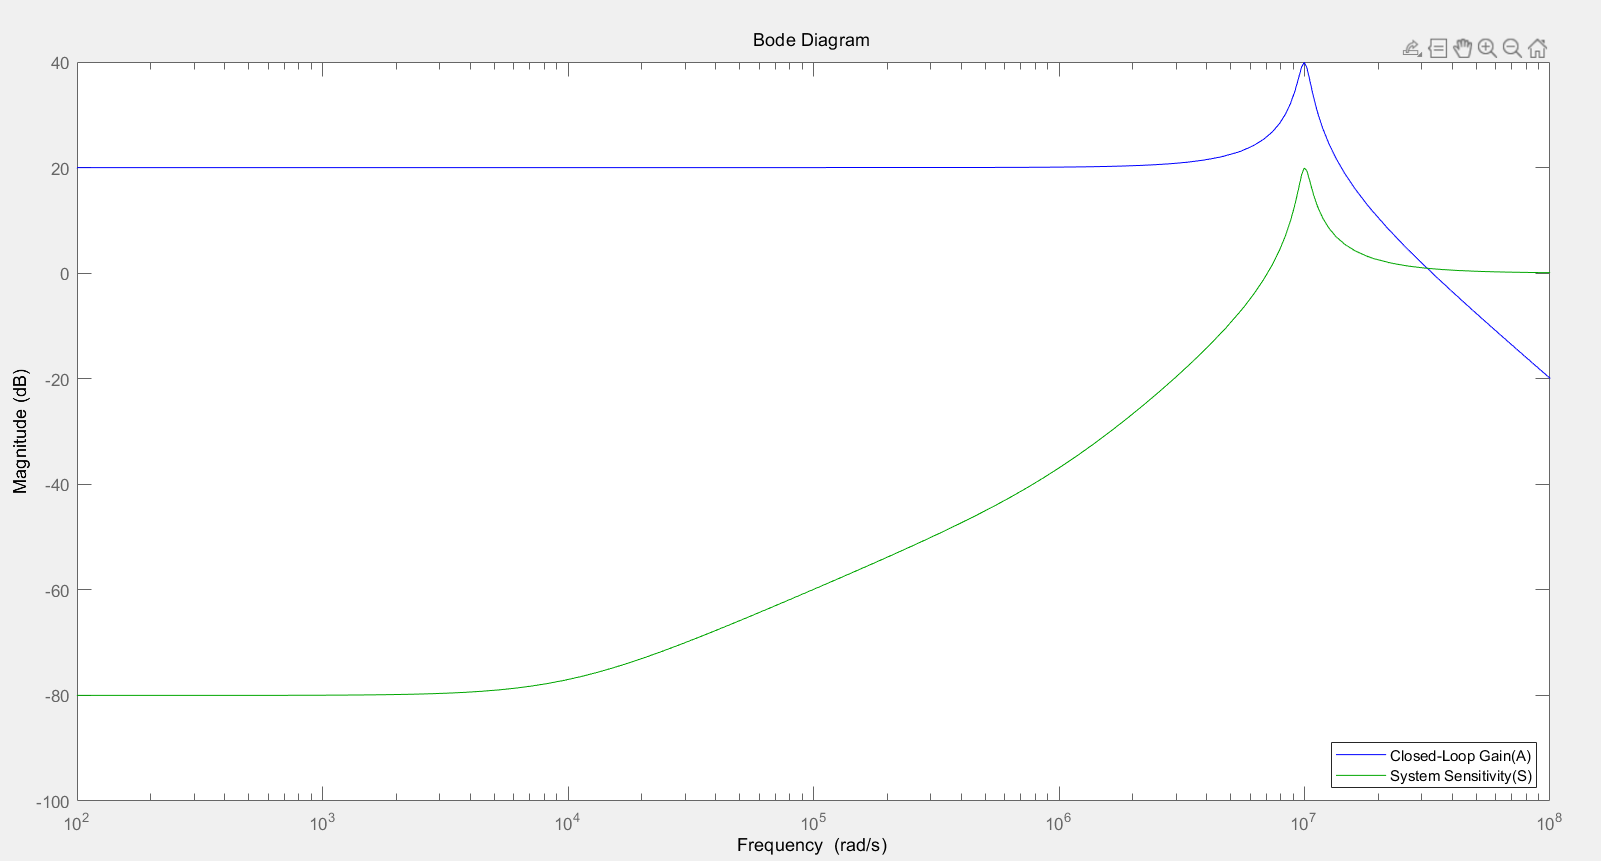
\includegraphics[keepaspectratio,width=500pt]{4.png}
    \caption{串联Washout滤波器的系统根轨迹图}
\end{figure}

这里我们取K=2.34,阻尼比为0.312,固定好增益,再次检查脉冲响应(图1.5)。

\begin{figure}[htbp]
    \centering
    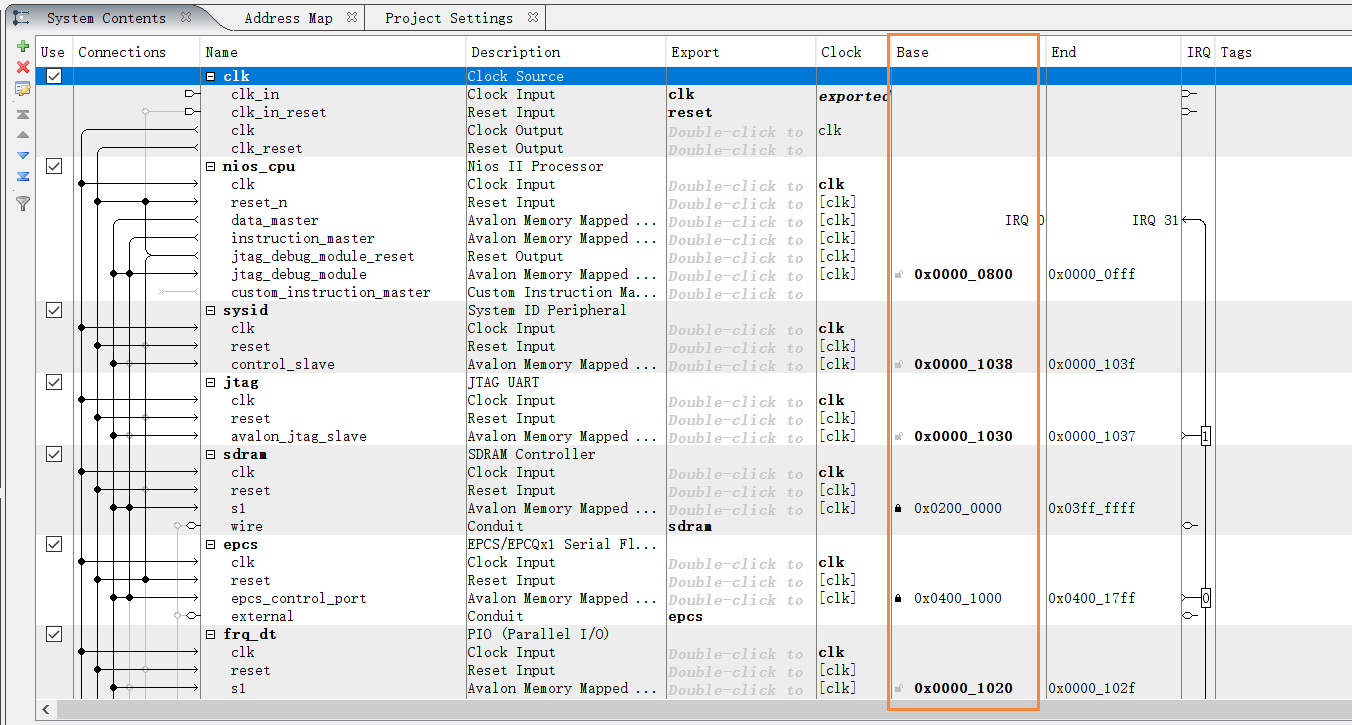
\includegraphics[keepaspectratio,width=500pt]{5.png}
    \caption{串联Washout滤波器的脉冲响应}
\end{figure}

再次观察副翼到倾斜角度的脉冲响应(图1.6)

\begin{figure}[htbp]
    \centering
    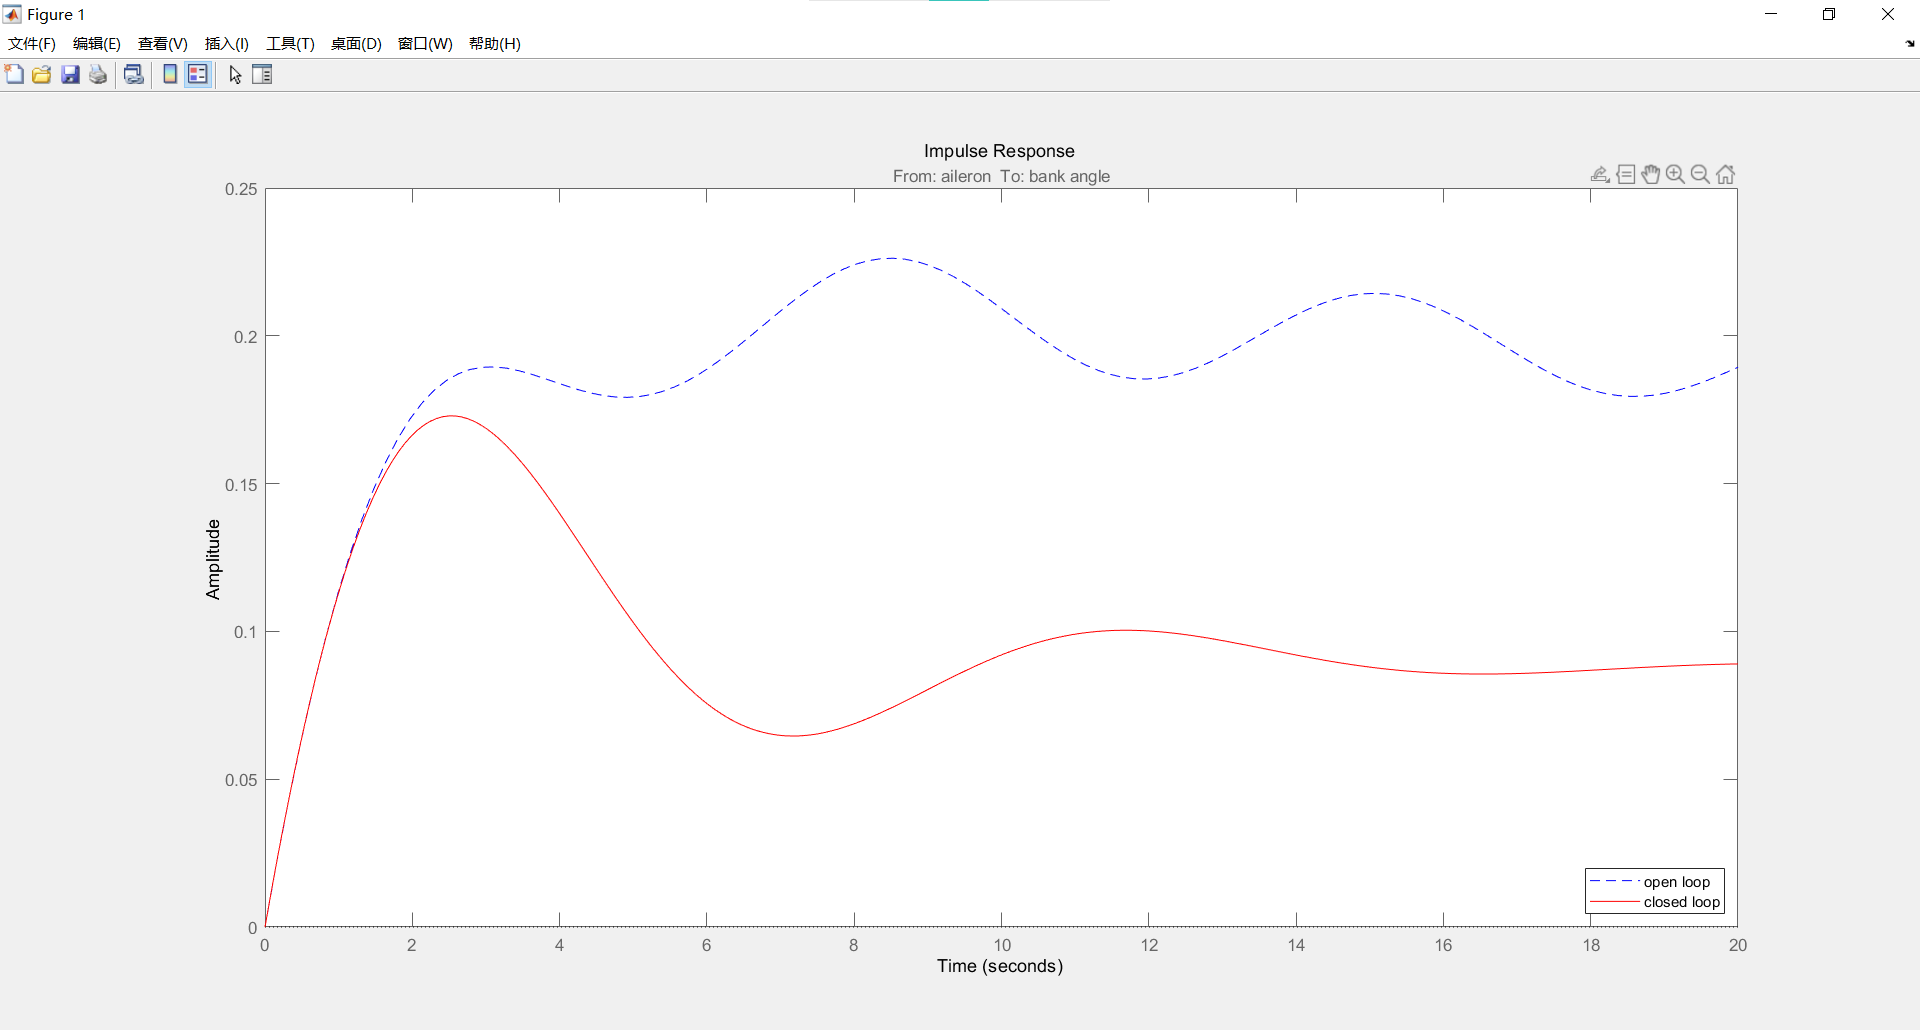
\includegraphics[keepaspectratio,width=500pt]{6.png}
    \caption{改进过后的副翼到倾斜角度的脉冲响应}
\end{figure}

发现倾斜和转向行为已经恢复正常。
最终的这个阻尼器就是我们最终设计的模型,我们发现虽然它不完全符合要求,但这种设计在大大增加了阻尼的同时,允许飞行员正常驾驶飞机。
在实际设计反馈系统时,要根据设计的需求设计对应的反馈效果,同时要考虑到现实因素,这样才能设计出能够付至使用的反馈系统。


\chapter{探究收获}
通过理解747喷气式飞机偏航阻尼器设计,我对自动控制系统的设计有了更深一步的了解,最大的收获是对实际情况中如何正确的运用自动控制理论去解决实际问题。
在课上学习到的各个知识点在设计过程中都有着很好的对应,使我的自动控制原理有了现实应用的照应,帮助我更好地理解自动控制原理的模型构建与分析。在实际设计中还要考虑反馈时的实际情况,不能脱离现实导致构建的模型违背实际应用。






\backmatter


% %=======%
% %引入参考文献文件
% %=======%
\bibdatabase{bib/POC}%bib文件名称 仅修改bib/ 后部分
\printbib
\nocite{*} %显示数据库中有的,但是正文没有引用的文献


% \Appendix

% 这里是附录页,可要可不要

% \Thanks.



\end{document}